\documentclass[xcolor=dvipsnames]{beamer}
% Class options include: notes, notesonly, handout, trans,
%                        hidesubsections, shadesubsections,
%                        inrow, blue, red, grey, brown

% Theme for beamer presentation.
\usetheme{Susan}

\usepackage{graphics}
\usepackage{multicol}
\usepackage{url}


\section*{Programs with Python}

\begin{document}

\begin{frame}
\begin{center}{\Huge Building Programs with Python}
\end{center}
\end{frame}


\begin{frame}[fragile]
For our Python introduction we're going to pretend to be a researcher named Harold Bridge (user id {\tt hbridge}) who is studying inflammation in patients who have been given a new treatment for arthritis.

Use Mercurial to grab the files from Bitbucket and put them in an {\tt hbridge} directory in your SWC workspace:
{\footnotesize
\begin{verbatim}
$ cd
$ cd Desktop/swc
$ hg clone https://bitbucket.org/douglatornell/swc-hbridge-files hbridge
\end{verbatim}
}

You can copy and paste the {\tt hg clone} command from the Etherpad.
\end{frame}


\begin{frame}
\frametitle{Analyzing Patient Data Part 1}
\begin{enumerate}
\item    Explain what a library is, and what libraries are used for.
\item    Load a Python library and use the things it contains.
\item    Read tabular data from a file into a program.
\item    Assign values to variables.
\item    Select individual values and subsections from data.
\end{enumerate}

\begin{multicols}{2}
\begin{itemize}
\item import numpy
\item numpy.loadtxt(fname=  delimiter=)
\item weight\_kg = 55
\item print
\item weight\_lb = 2.2 * weight\_kg
\item type(data)
\item data.shape
\item data[0,0], data[0:1,0:1]
\item data[0:10:2,1]
\item data[:3,36:]
\end{itemize}
\end{multicols}
\end{frame}

\begin{frame}
\frametitle{Analyzing Patient Data Part 2}
\begin{enumerate}
\setcounter{enumi}{5}
\item    Perform operations on arrays of data.
\item    Display simple graphs.
\end{enumerate}
\begin{multicols}{2}
\begin{itemize}
\item data.mean()
\item data.std()
\item data.mean(axis=0)
\item \%matplotlib inline
\item from matplotlib import pyplot
\item pyplot.imshow(data)
\item pyplot.show()
\item pyplot.plot(ave\_inflammation)
\item import matplotlib import pyplot as plt
\item plt.subplot(1,3,1)
\item plt.ylabel('average')
\item plt.show()
\end{itemize}
\end{multicols}
\end{frame}


\begin{frame}
\frametitle{Exercise}
Create a single plot showing 1) the mean for each day and 2) the mean + 1 standard deviation for each day and the 3) the mean - 1 standard deviation for each day.
\end{frame}

\begin{frame}[fragile]
\frametitle{Creating Functions Part 1}
\begin{enumerate}
\item    Define a function that takes parameters.
\item    Return a value from a function.
\item    Test and debug a function.
\end{enumerate}
\begin{itemize}
\item
\begin{verbatim}
def fahr_to_kelvin(temp):
     return ((temp - 32) * (5/9)) + 273.15
\end{verbatim}
\item from \_\_future\_\_ import division
\item
\begin{verbatim}
def kelvin_to_celsius(temp):
    return temp - 273.15
\end{verbatim}
\item
\begin{verbatim}
def fahr_to_celsius(temp):
    temp_k = fahr_to_kelvin(temp)
    result = kelvin_to_celsius(temp_k)
    return result
\end{verbatim}
\end{itemize}
\end{frame}

\begin{frame}
\frametitle{Creating Functions Part 2}
\begin{enumerate}
\setcounter{enumi}{3}
%\item    Explain what a call stack is, and trace changes to the call stack as functions are called.
\item    Explain the scope of a variable and the idea of encapsulation.
\end{enumerate}
\resizebox{\textwidth}{!}{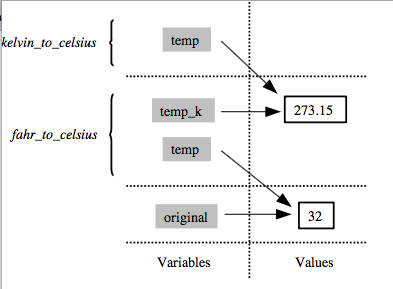
\includegraphics{img/python-call-stack-05.png}}
\end{frame}


\begin{frame}[fragile]
\frametitle{Creating Functions Part 3}
\begin{enumerate}
\setcounter{enumi}{2}
\item    Test and debug a function.
\item    Explain why we should divide programs into small, single-purpose functions.
\end{enumerate}
\begin{itemize}
\item
\begin{verbatim}
def centre(data, desired):
    return (data - data.mean()) + desired
\end{verbatim}
\item z = numpy.zeros((2,2))
\item print centre(z, 3)
\item print data.std() - centred.std()
\item '''centre(data, desired): return a new array containing the original data centered around the desired value.'''
\item help(centre)
\end{itemize}
\end{frame}

\begin{frame}
\frametitle{Exercise}
Write a function called analyze that takes a filename as a parameter and displays the three graphs produced in the previous lesson, i.e., analyze('inflammation-01.csv') should produce the graphs already shown, while analyze('inflammation-02.csv') should produce corresponding graphs for the second data set. Be sure to give your function a docstring. Hint: a function can just ``do'' something.  It doesn't necessarily need to return anything.
\end{frame}



\begin{frame}[fragile]
\frametitle{Creating Functions Part 4}
\begin{enumerate}
\setcounter{enumi}{5}
\item    Set default values for function parameters.
\end{enumerate}
\begin{itemize}
\item def center(data, desired = 0):
\item
\begin{verbatim}
def display(a=1, b=2, c=3):
    print 'a:', a, 'b:', b, 'c:', c

print 'no parameters:'
display()
print 'one parameter:'
display(55)
print 'two parameters:'
display(55, 66)
\end{verbatim}
\item help(numpy.loadtxt)
\end{itemize}
\end{frame}

\begin{frame}[fragile]
\frametitle{Analyzing Multiple Data Sets: Part 1}
You should have a working function analyze.  If not, its at the top of
\url{https://douglatornell.github.io/2014-09-25-ubc/novice/python/03-loop.html}
\begin{enumerate}
\item    Explain what a for loop does.
\item    Correctly write for loops to repeat simple calculations.
\end{enumerate}
\begin{itemize}
\item
\begin{verbatim}
def print_characters(element):
    print element[0]
    print element[1]
    print element[2]
\end{verbatim}
\item print\_characters('tin')
\item print\_characters('hg')
\item
\begin{verbatim}
def print_characters(element):
    for char in element:
        print char
\end{verbatim}
\end{itemize}
\end{frame}

\begin{frame}[fragile]
\frametitle{Analyzing Multiple Data Sets: Part 2}
\begin{enumerate}
\setcounter{enumi}{2}
\item    Trace changes to a loop variable as the loop runs.
\item    Trace changes to other variables as they are updated by a for loop.
\end{enumerate}
\begin{itemize}
\item
\begin{verbatim}
length = 0
for vowel in 'aeiou':
    length = length + 1
print 'There are', length, 'vowels'
\end{verbatim}
\item
\begin{verbatim}
letter = 'z'
for letter in 'abc':
    print letter
print 'after the loop, letter is', letter
\end{verbatim}
\item len('aeiou')
\end{itemize}
\end{frame}

\begin{frame}
\frametitle{Analyzing Multiple Data Sets: Part 3}
\begin{enumerate}
\setcounter{enumi}{4}
\item     Explain what a list is.
\item    Create and index lists of simple values.
\end{enumerate}
\begin{multicols}{2}
\begin{itemize}
\item odds = [1,3,5,7]
\item odds[0], odds[-1]
\item for number in odds:
\item names = ['Newton', 'Darwig', 'Turing']
\item names[1] = 'Darwin'
\item name = 'Darwig'
\item name[5] = 'n'
\item odds.append[9]
\item del odds[0]
\item odds.reverse()
\end{itemize}
\end{multicols}
\end{frame}

\begin{frame}
\frametitle{Exercise}
Write a function called total that calculates the sum of the values in a list. (Python has a built-in function called sum that does this for you. Please don't use it for this exercise.)
\end{frame}

\begin{frame}[fragile]
\frametitle{Analyzing Multiple Data Sets: Part 4}
\begin{enumerate}
\setcounter{enumi}{6}
\item     Use a library function to get a list of filenames that match a simple wildcard pattern.
\item    Use a for loop to process multiple files.
\end{enumerate}
\begin{itemize}
\item import glob
\item print glob.glob('*.ipynb')
\item
\begin{verbatim}
filenames = glob.glob('*.csv')
filenames = filenames[0:3]
for f in filenames:
    print f
    analyze(f)
\end{verbatim}
\end{itemize}
\end{frame}


\begin{frame}
\frametitle{Conditionals -- Making Choices}
\begin{enumerate}
  \item Write conditional statements including {\tt if}, {\tt elif}, and {\tt else} branches.
  \item Correctly evaluate expressions containing {\tt and} and {\tt or}.
  \item Correctly write and interpret code containing nested loops and conditionals.
\end{enumerate}
\begin{multicols}{2}
\begin{itemize}
  \item {\tt numpy.empty()}
  \item {\tt numpy.empty\_like()}
  \item {\tt +=, -=, *=, /=}
  \item {\tt if ... elif ... else}
  \item {\tt ==, !=, <, <=, >, >=}
  \item {\tt and, or, not}
  \item non-printing characters; e.g. \textbackslash{\tt n}
  \item Line continuations in code
\end{itemize}
\end{multicols}
\end{frame}


\begin{frame}
\frametitle{Python Modules and Command-line Programs}
\begin{enumerate}
  \item Create a Python module containing functions that can be `import`-ed into notebooks and other modules.
  \item Use the values of command-line arguments in a program.
  \item Read data from standard input in a program so that it can be used in a pipeline.
\end{enumerate}
\begin{multicols}{2}
\begin{itemize}
  \item {\tt \%\%writefile}
  \item {\tt !cat}
  \item Module \& function docstrings
  \item {\tt reload()}
  \item {\tt sys.argv}
  \item {\tt \$ python myfile.py}
  \item {\tt if \_\_name\_\_ == "\_\_main\_\_":}
  \item {\tt sys.stdin}
  \item {\tt argparse}
\end{itemize}
\end{multicols}
\end{frame}

\end{document}
